\documentclass{article}

\usepackage{color}
\usepackage{graphicx}
\usepackage{tabularx}


\usepackage{geometry}
 \geometry{
 top=20mm,
 bottom=20mm,
 }


\title{Document de présentation}
\author{Justal Kevin}
\date{26/09/2015}
\renewcommand{\contentsname}{Table des matières} 
 
\newcommand\invisiblesection[1]{%
  \refstepcounter{section}%
  \addcontentsline{toc}{section}{\protect\numberline{\thesection}#1}%
  \sectionmark{#1}} 
 
\begin{document}

\begin{center}
\textbf{\Huge{LES ANIMAUX}}
\line(1,0){300}\\
DOSSIER DE CONCEPTION\\
\vspace{3cm}
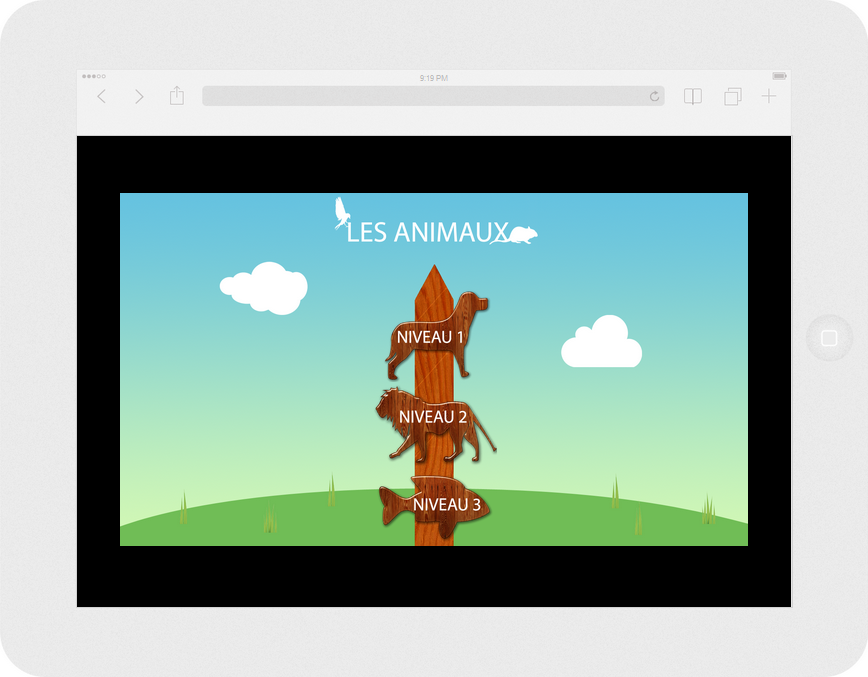
\includegraphics[width=0.8\textwidth]{tablette}\\
\vspace{3cm}
\textbf{Justal Kevin - \color{blue}{\underline{justal@polytech.unice.fr}} \color{black}{- SI5 - IHM}}\\
\textbf{Houda Smach - \color{blue}{\underline{smach.houda@gmail.com}} \color{black}{- SSTIM }}\\
\textbf{Belokogne Ivan - \color{blue}{\underline{bel.ivan@live.com }} \color{black}{- SSTIM }}\\
\vspace{4cm}
\textbf{Encadrant :}\\
\textbf{Jean-Paul Stromboni - \color{blue}{\underline{strombon@polytech.unice.fr}}}
\end{center}

\newpage
\tableofcontents

\newpage

\section{Présentation de l'application}
\hspace*{0.6cm}Les jeux accessibles sont un bon moyen d'aider le développement intellectuel et psychologique des enfants handicapés. C'est pour cela que nous avons décidé de produire un jeu le plus simple possible faisant travailler l'intelligence logico-mathématique et corporelle kinesthésique des enfants. Le jeu confronte les enfants à plusieurs images d'animaux et des cases où chaque animal peut être rangé. Les enfants devront donc associer des animaux ayant le même nombre de pattes, le même type d'habitation ou encore la même catégorie (domestique, de la ferme, sauvage).
\section{Structure de l'application}

\subsection{Déroulement}

La structure génerale de notre application sera la suivante :
\vspace{0.5cm}\\
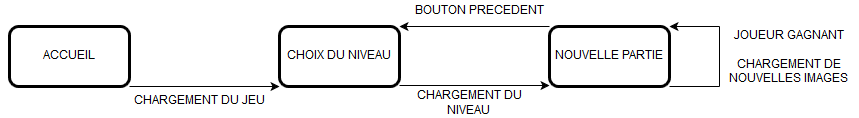
\includegraphics[width=\textwidth]{plan}
\vspace{0.5cm}\\
\hspace*{0.6cm}La structure est volontairement simple afin que toute personne puisse prendre le jeu en main sans aucune indication.\\
Une fois la page d'accueil chargée, le choix des différents niveaux s'affiche. Lorsque l'utilisateur clique sur l'une des options, le jeu lance le niveau selectionné.\\
Si l'utilisateur décide d'arrêter le jeu ou de changer de niveau, il peut alors revenir au menu du départ en cliquant sur le bouton "retour". 

\subsection{UML}

\begin{center}
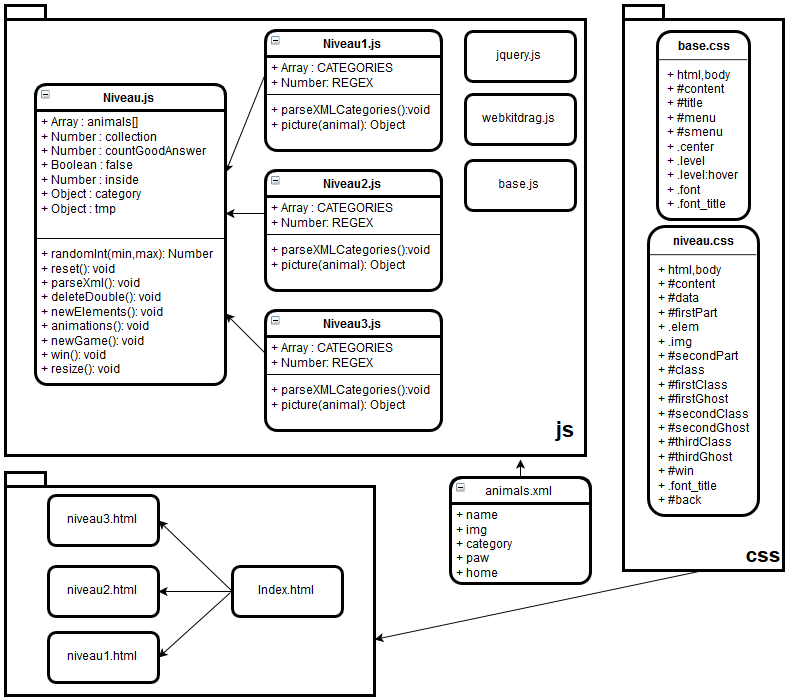
\includegraphics[width=0.8\textwidth]{planUml}\\
\end{center}

\section{Interfaces}
\hspace*{0.6cm}Le jeu dispose de quatre scènes clés qui à elles seules suffisent pour décrire le jeu entier. Dans chaque section du jeu, nous verrons en détail les objectifs et les accomplissements que l'on attend du joueur. 
\subsection{Ecran d'accueil}
\vspace{0.5cm}
\begin{center}
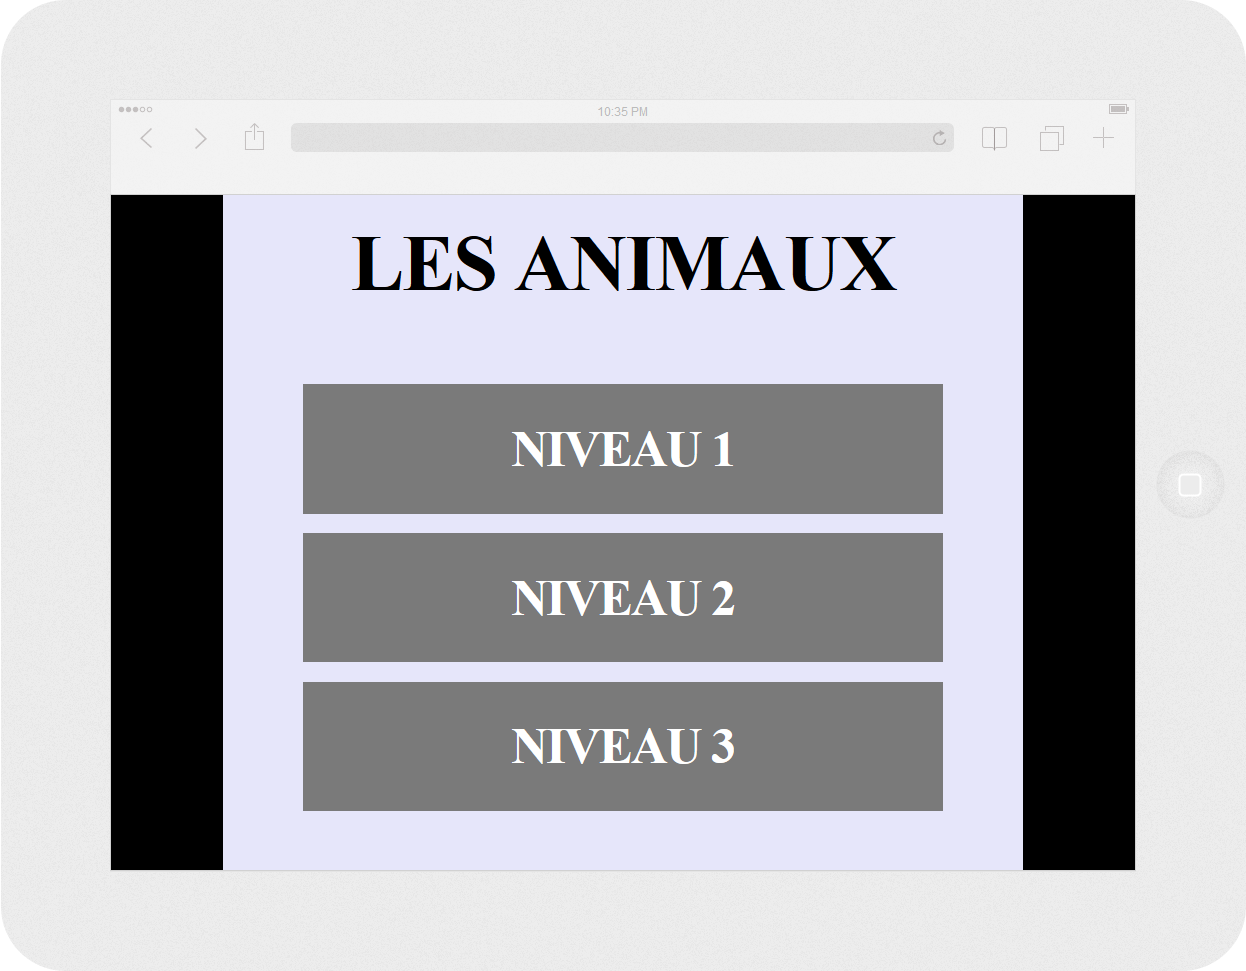
\includegraphics[width=0.6\textwidth]{page1}
\end{center}
\vspace{0.5cm}
\hspace*{0.6cm}Le menu est très simple, épuré de tout contenu additionnel inutile. Le texte est écrit très gros au cas où l'enfant aurait un handicap visuel. De même pour éviter que l'enfant ouvre les options du navigateur au cas où le jeu serait lancé sur un ordinateur, le clic droit a été désactivé. The cursor a aussi été modifié, il est beaucoup plus grand que la normal pour l'enfant atteint d'un handicap visuel.
\vspace{0.5cm}\\
\hspace*{0.6cm}Sinon concernant le menu, il y a le minimum d'animation pour que le joueur puisse s'y retrouver. Lorsque le joueur passe la souris sur les différents niveaux, ces derniers sont surlignés et grossis légèrement.
\subsection{Niveau 1 - Trier par catégories}
\vspace{0.5cm}
\begin{center}
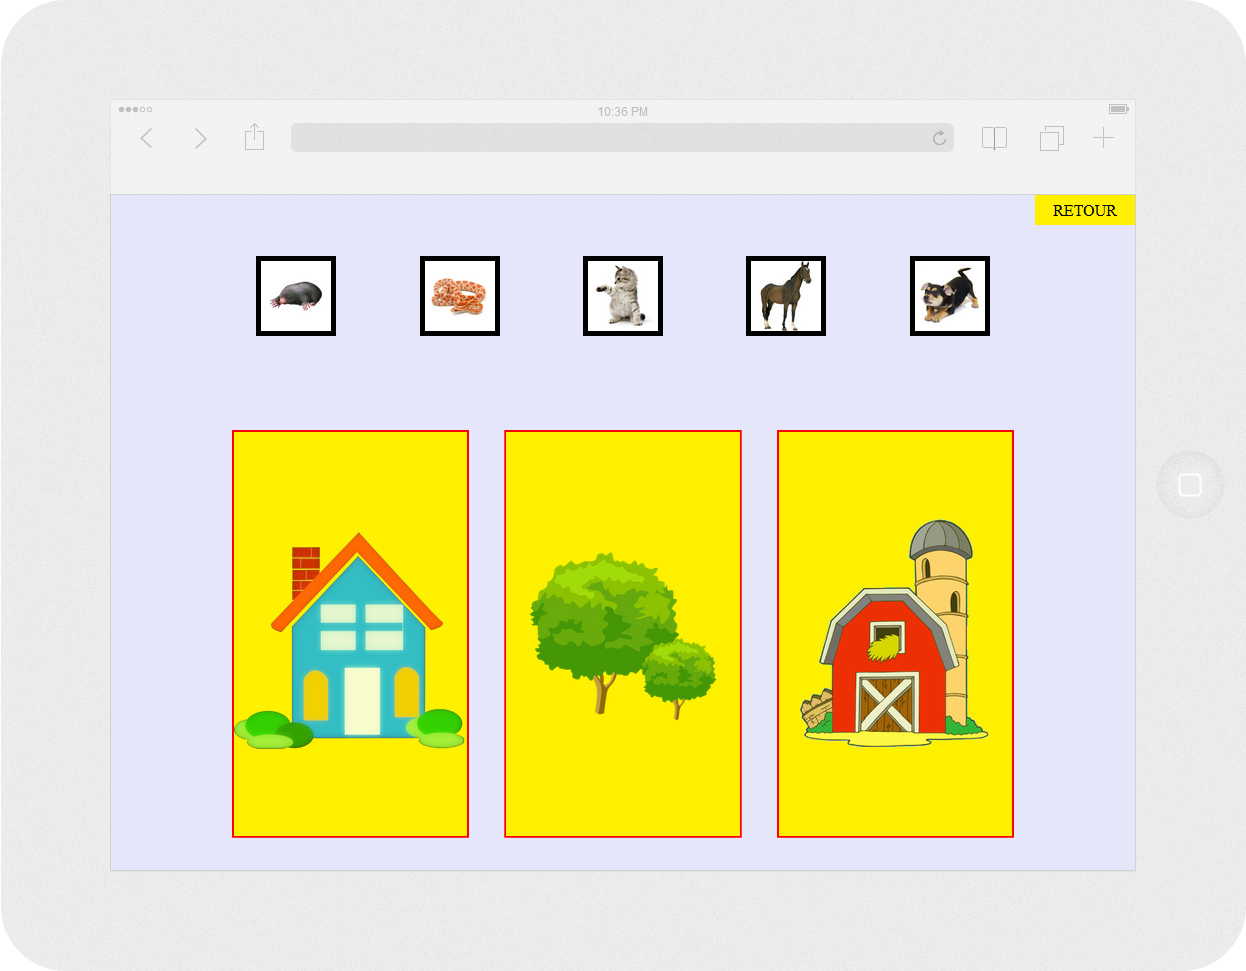
\includegraphics[width=0.6\textwidth]{page2}
\end{center}
\vspace{0.5cm}
\hspace*{0.6cm}Comme l'ensemble du jeu, les niveaux sont eux aussi simplifiés au maximum.
Le premier niveau consiste à associer les animaux affichés à leurs catégories respectives. Prenons un exemple, un chat ira dans la catégorie domestique. On glisse alors l'image du chat sur la case jaune qui contient une maison. En cas de bonne réponse, l'image reste dans la case prévue. En cas de mauvaise réponse, l'image retourne à son emplacement d'origine.
\subsection{Niveau 2 - Trier par nombre de pattes}
\vspace{0.5cm}
\begin{center}
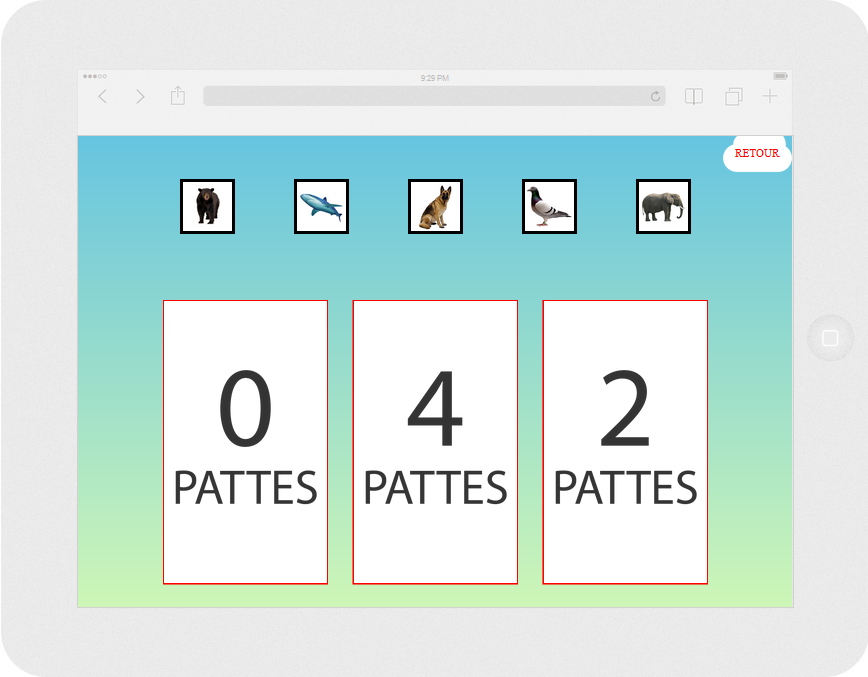
\includegraphics[width=0.6\textwidth]{page3}
\end{center}
\vspace{0.5cm}
\hspace*{0.6cm}Le niveau 2 est semblable au premier dans sa structure mais le jeu est plus difficile que le niveau 1. Dans ce niveau, le joueur doit trier les animaux par nombre de pattes. Par exemple, la case jaune avec le chien est la case qui regroupe les animaux avec 4 pattes comme le chat.
\subsection{Niveau 3 - Trier par habitation}
\vspace{0.5cm}
\begin{center}
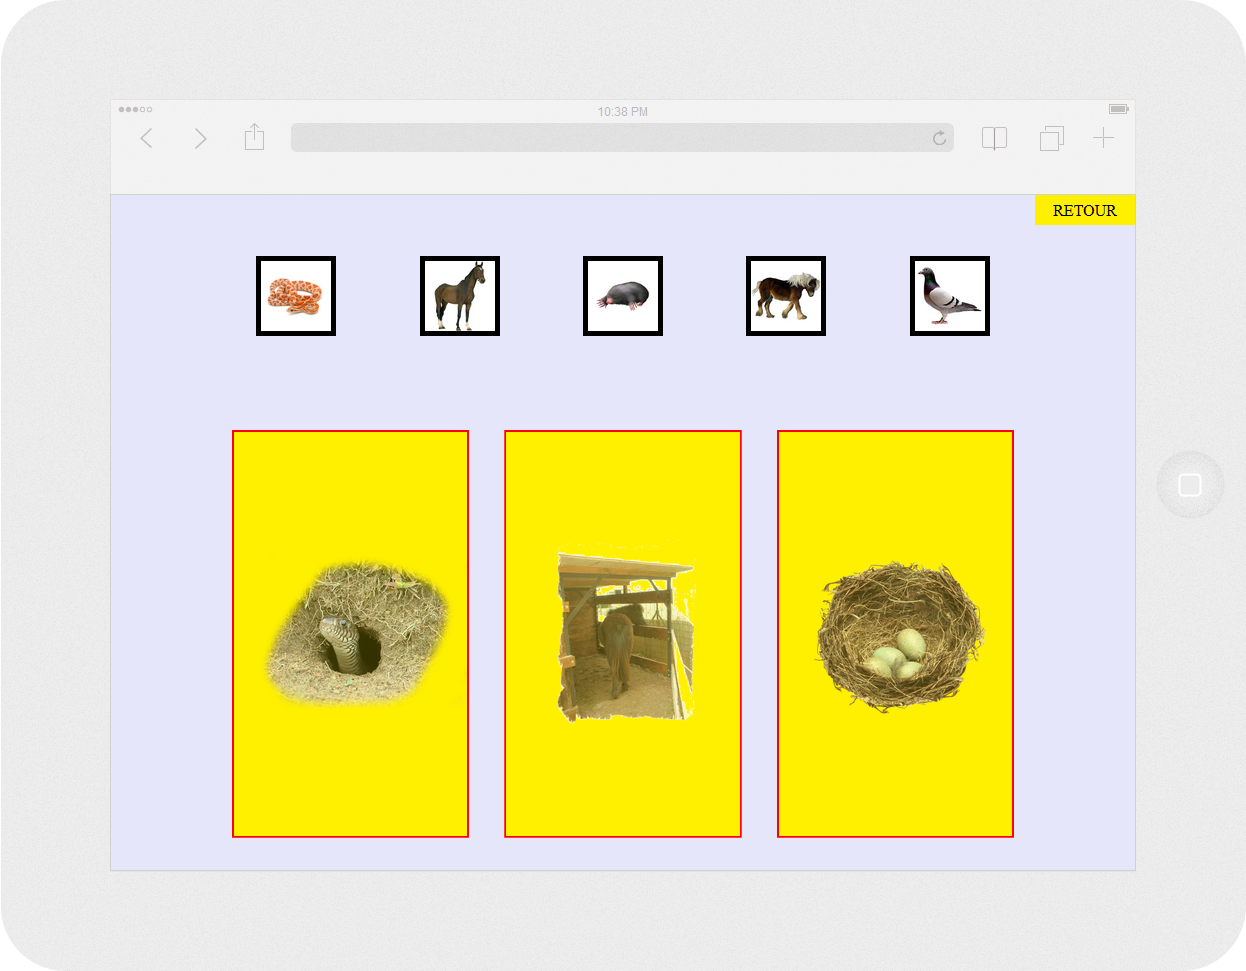
\includegraphics[width=0.6\textwidth]{page4}
\end{center}
\vspace{0.5cm}
\hspace*{0.6cm}Le dernier niveau est le plus difficile de tous. Cependant la structure et le gameplay restent là aussi similaires aux deux niveaux précédents. Seules les associations avec les animaux diffèrent. Cette fois, les animaux sont triés suivant leur habitats. Pour continuer avec les exemples, prenons le cheval, ce dernier vit dans une écurie. On déplacera donc l'image du cheval dans la case représentant l'écurie.
    
\section{Scénario}

Le jeu est composé de deux parties. En haut (zone1 en rouge), vous trouverez les animaux que vous pouvez déplacer et en bas (zone 2 en violet) les zones où vous pouvez les déplacer.
\vspace{0.5cm}\\
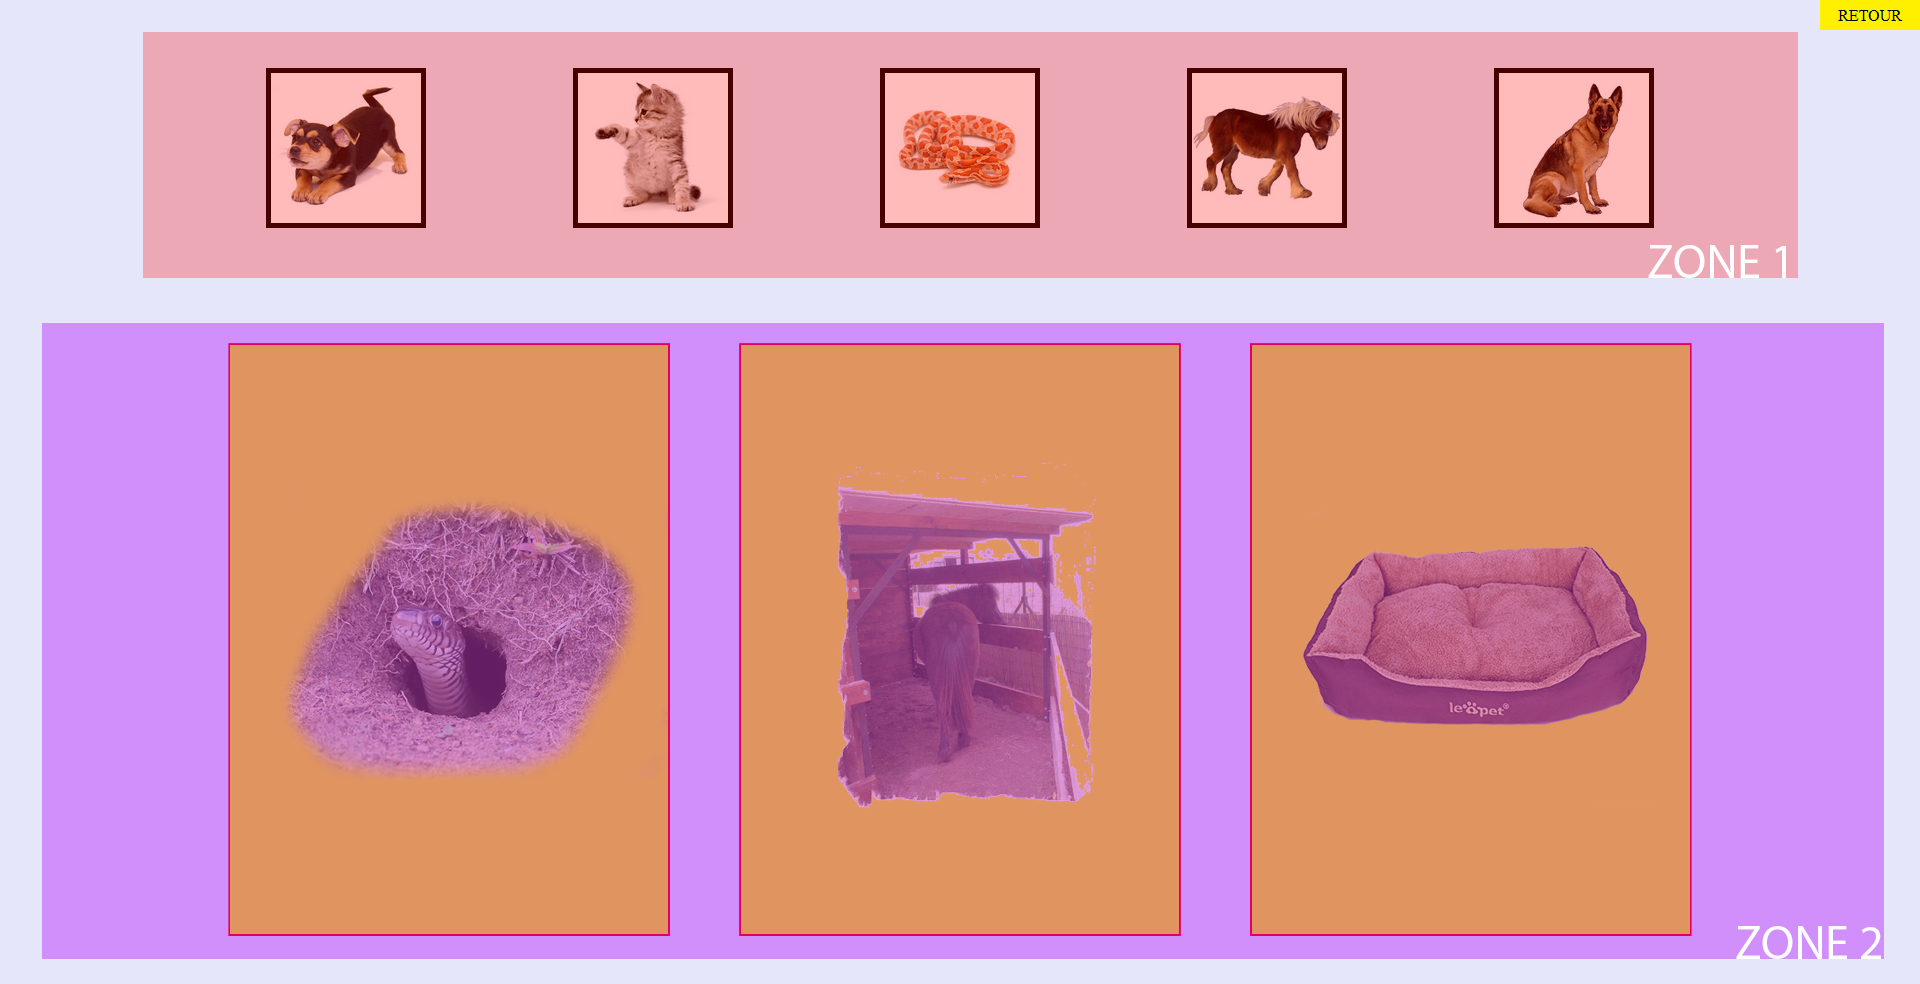
\includegraphics[width=1.0\textwidth]{zone}
\vspace{0.5cm}\\
Le but du jeu est de déplacer les animaux de la zone 1 vers la zone 2 en suivant une certaine logique. Reprenons notre exemple précédent et notons les animaux de la zone 1.\\
\vspace{0.5cm}\\
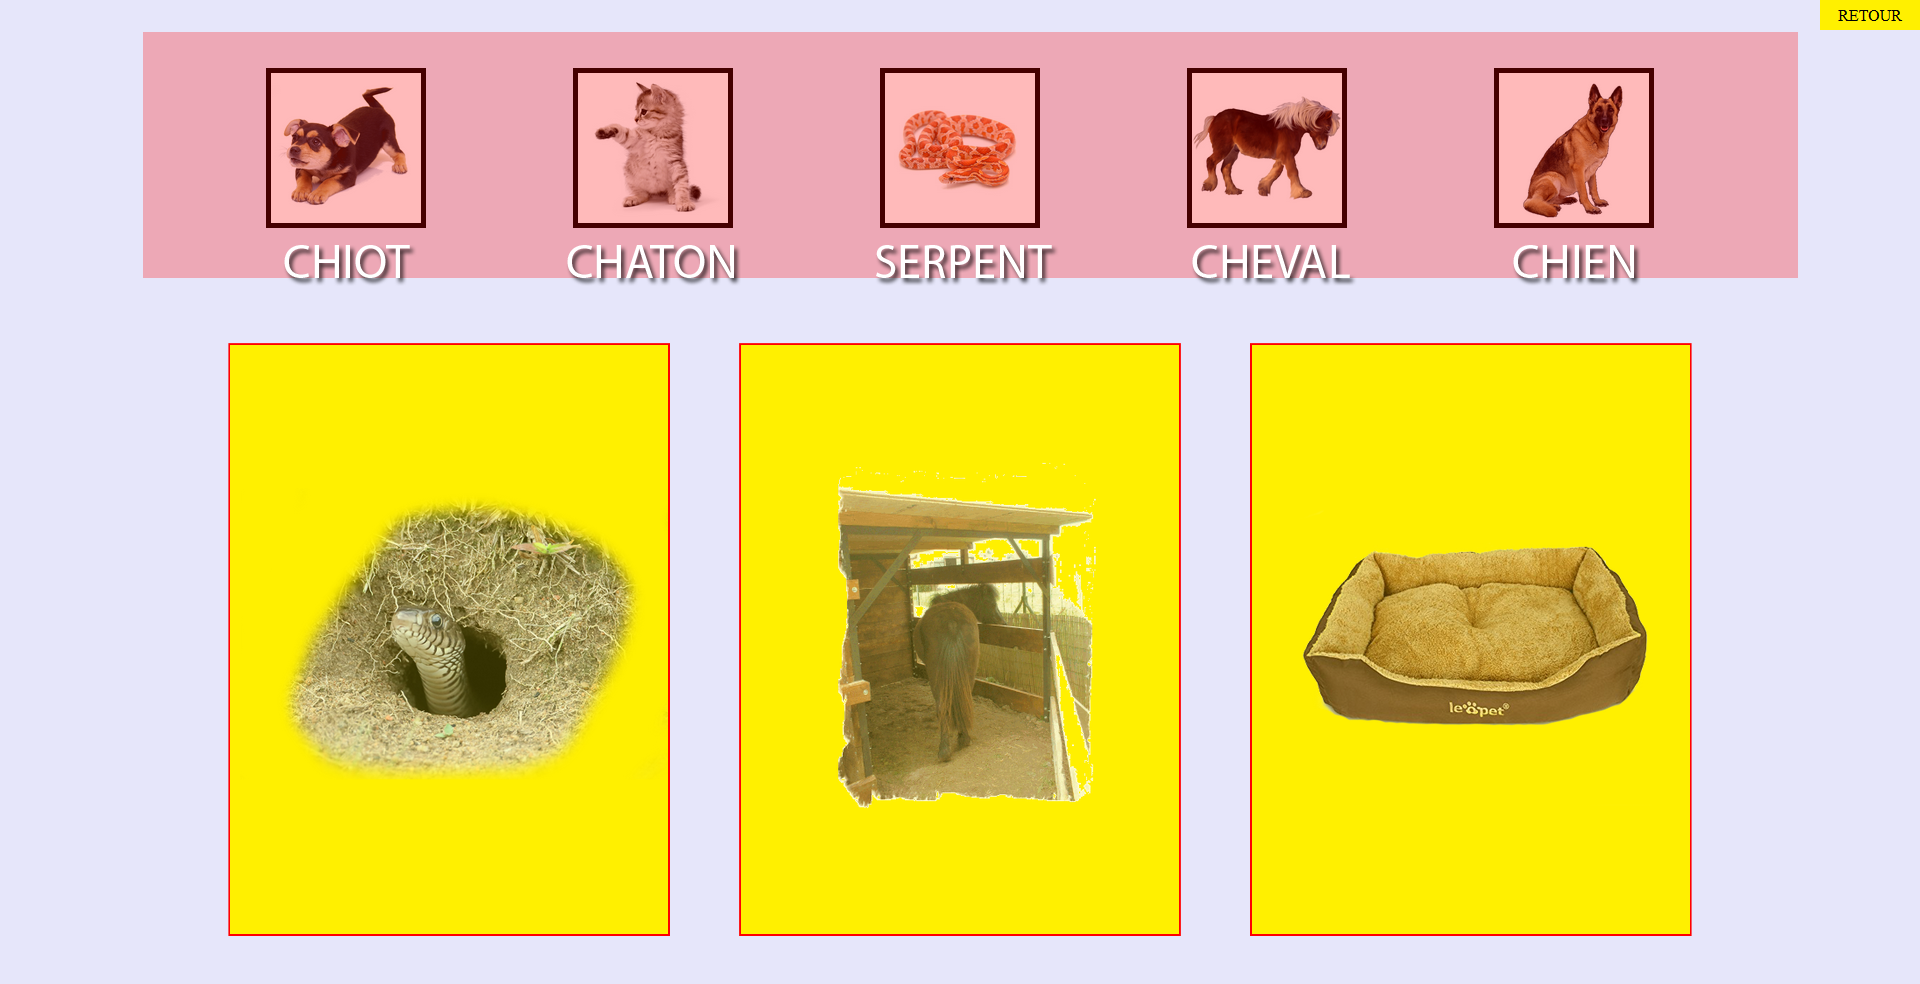
\includegraphics[width=1.0\textwidth]{zone1}
\vspace{0.5cm}\\
Prenons par exemple le cheval, nous allons cliquer dessus et maintenir notre clic tout en dépla\c{c}ant la souris.
\vspace{0.5cm}\\
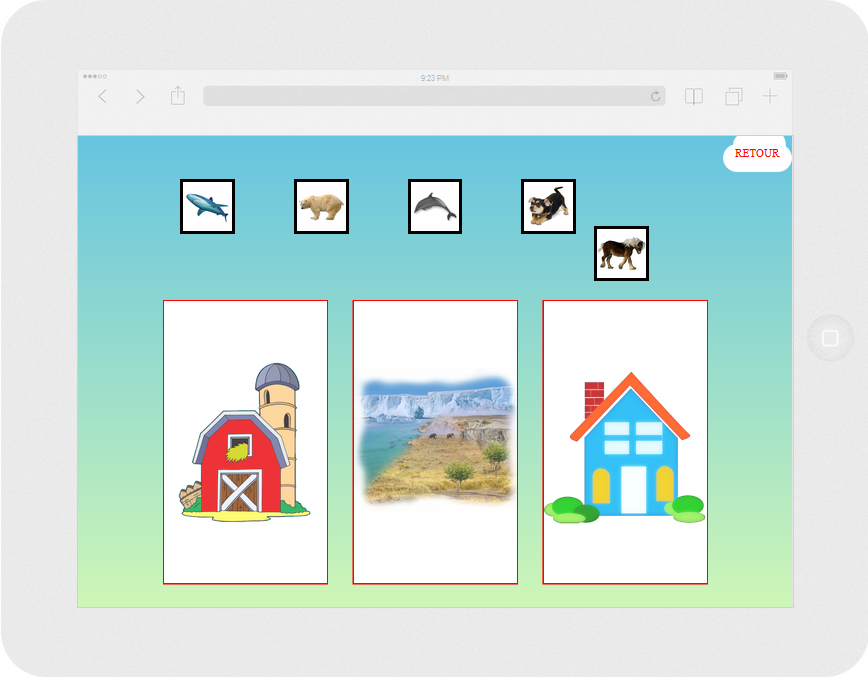
\includegraphics[width=1.0\textwidth]{zone2}
\vspace{0.5cm}\\
Si nous rel\^achons notre clic, l'image du cheval retournera à sa place automatiquement. Maintenant, regardons avec attention la zone 2 et décrivons là aussi les images. 
\vspace{0.5cm}\\
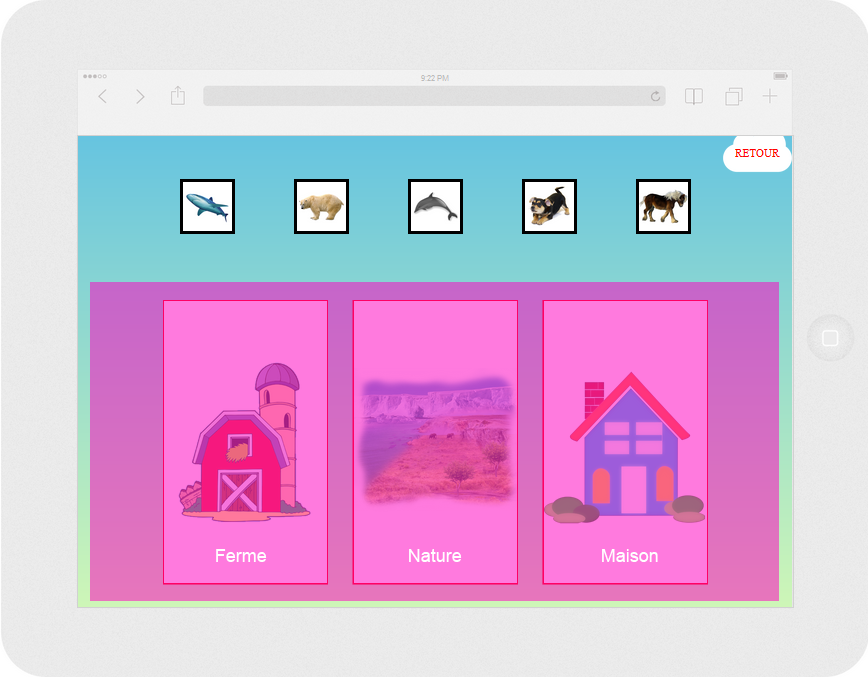
\includegraphics[width=1.0\textwidth]{zone3}
\vspace{0.5cm}\\
Reprenons maintenant notre cheval et dépla\c{c}ons le dans la zone qui lui correspond (l'écurie). L'image se fixera alors à la zone et vous ne pourrez plus y toucher. Vous avez la bonne réponse !
\vspace{0.5cm}\\
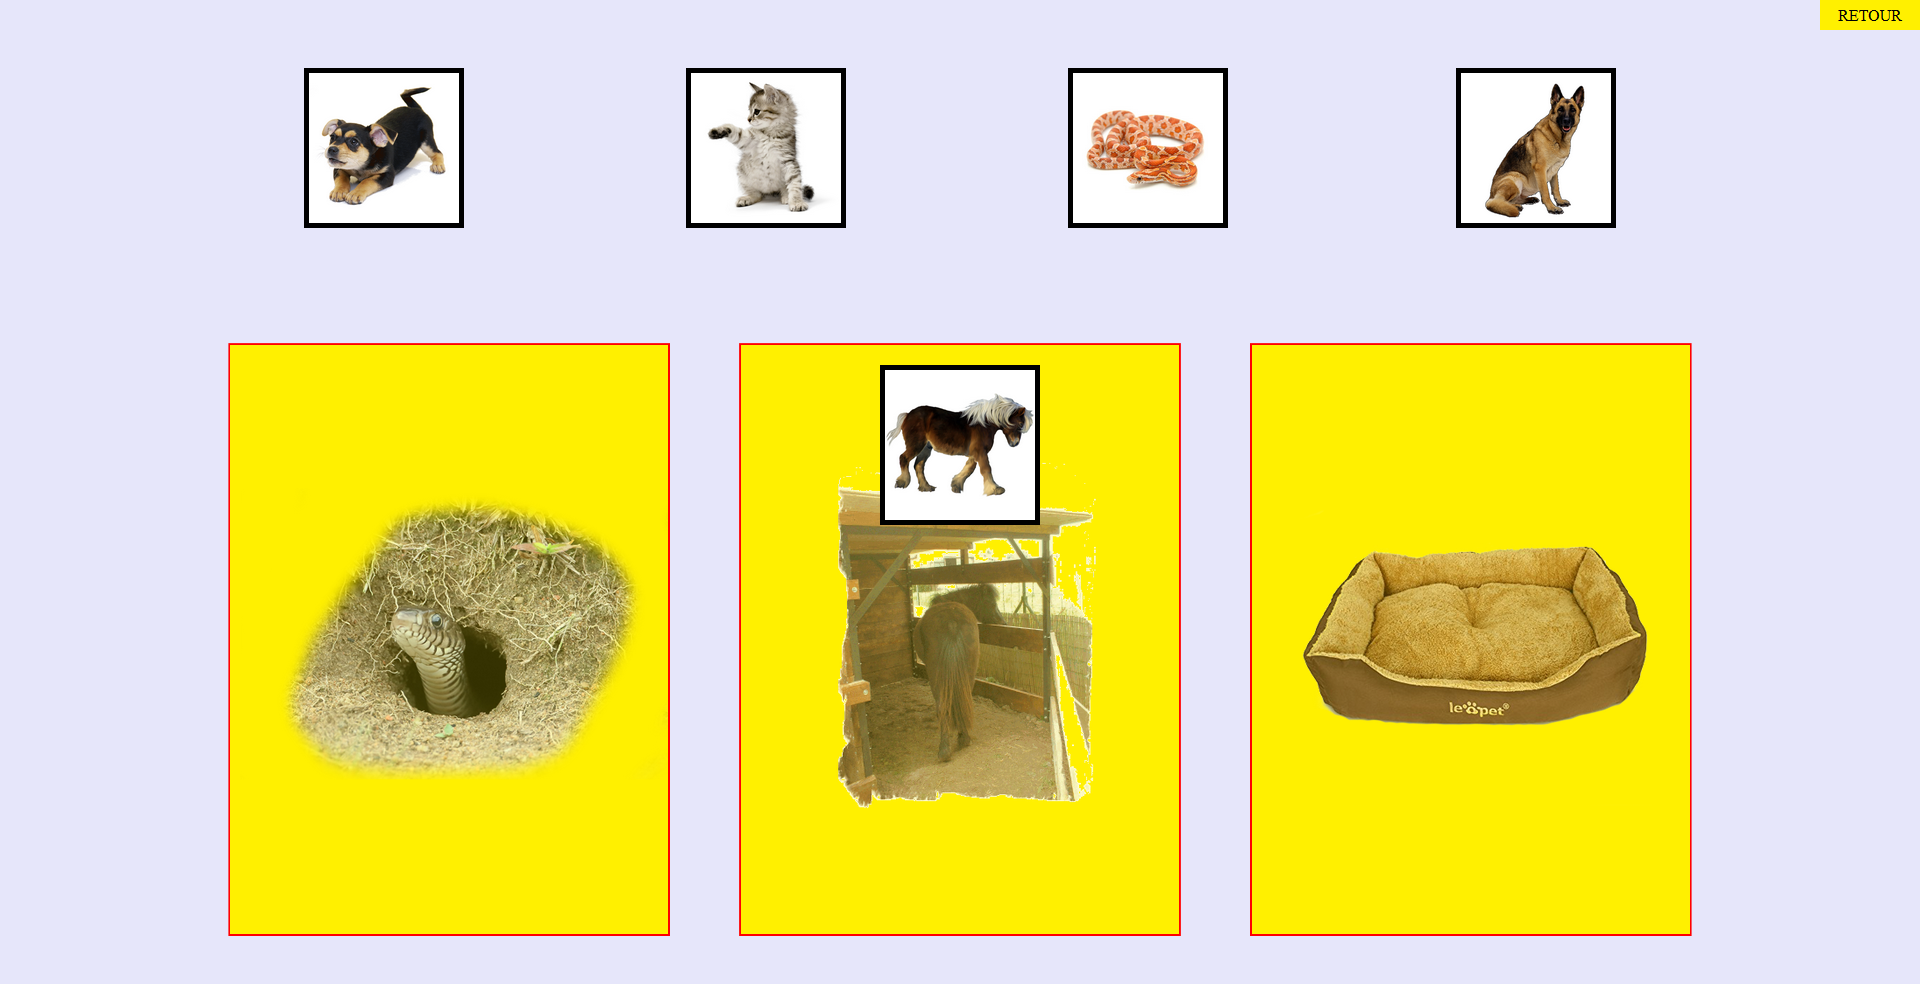
\includegraphics[width=1.0\textwidth]{zone4}
\vspace{0.5cm}\\
Maintenant effectuons cette même opération pour chaque image restante dans la zone 1. Allez, encore un petit effort, nous y somme presque.
\vspace{0.5cm}\\
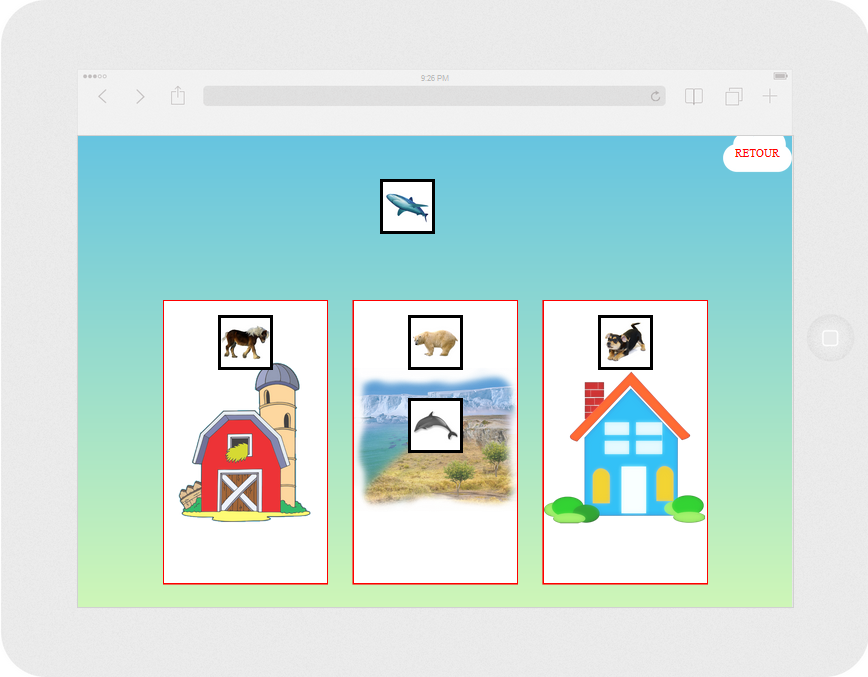
\includegraphics[width=1.0\textwidth]{zone5}
\vspace{0.5cm}\\
Si vous répondez correctement en pla\c{c}ant l'integralité des images, un message vous disant "Bravo" s'affiche alors pour vous féliciter.
\vspace{0.5cm}\\
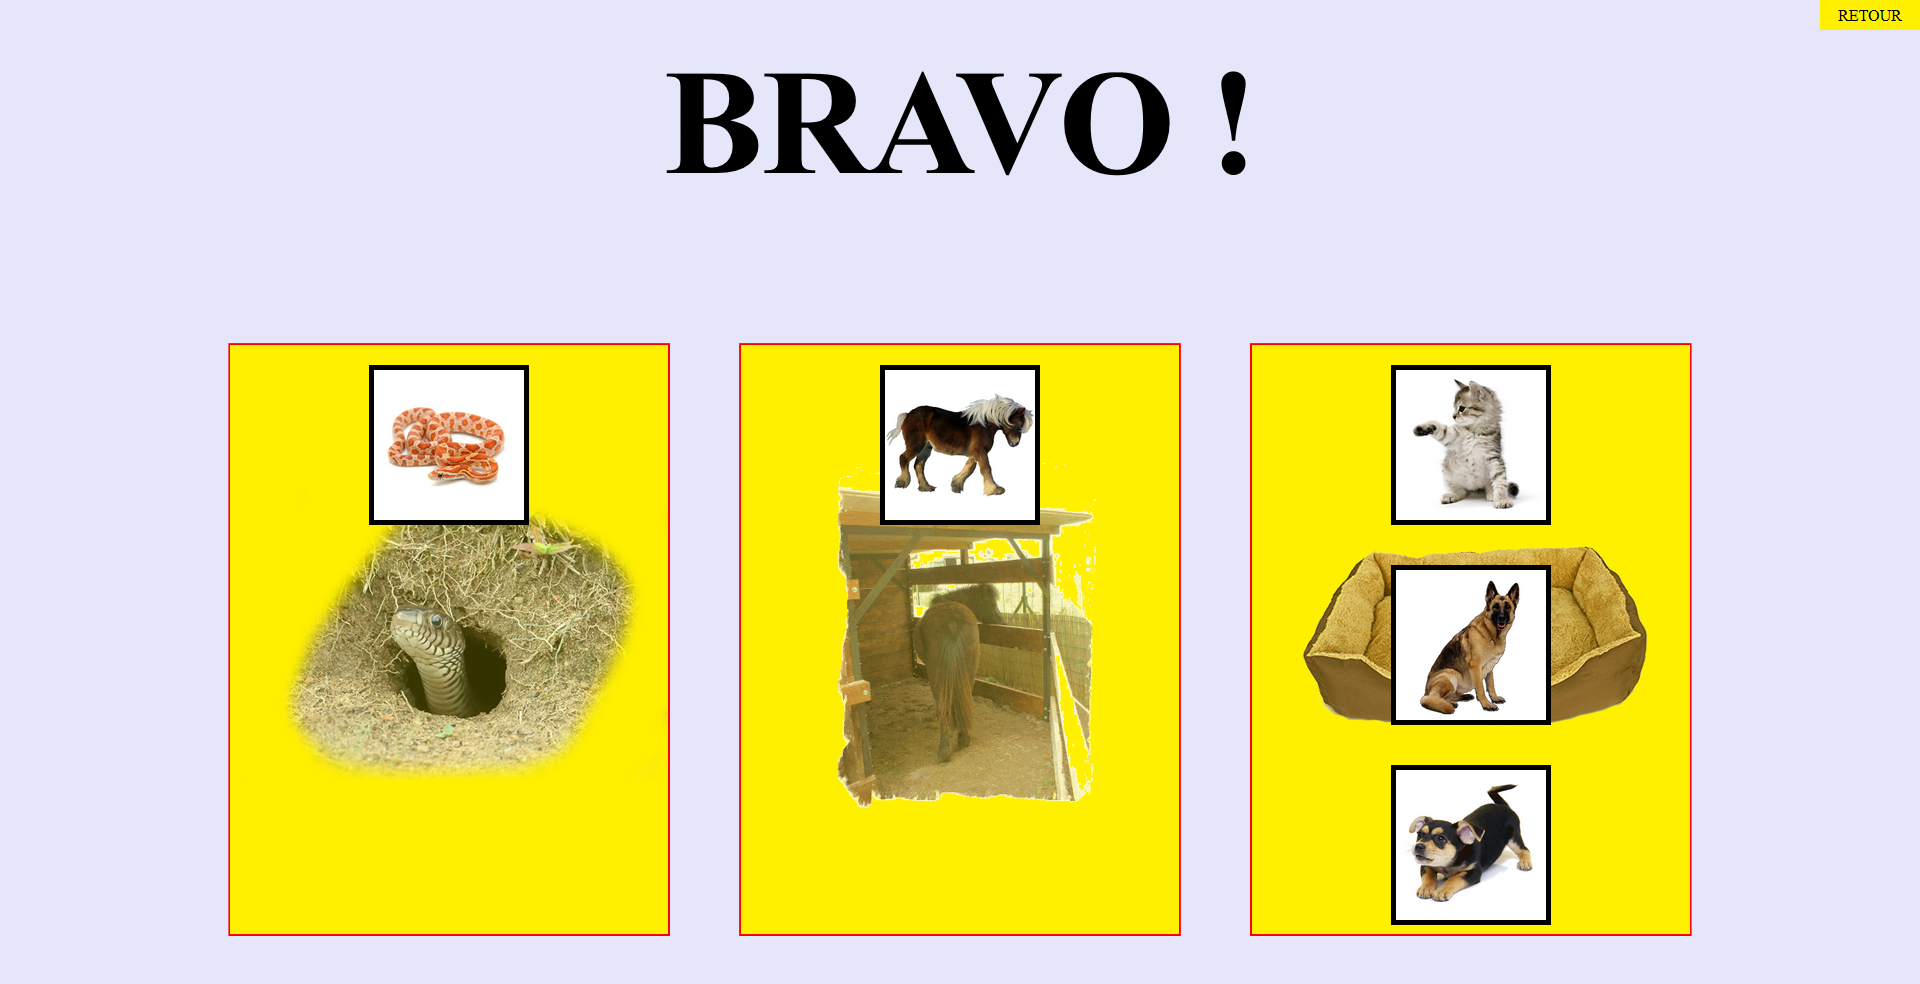
\includegraphics[width=1.0\textwidth]{zone6}
\vspace{0.5cm}\\
Puis une nouvelle partie commence avec de nouveaux éléments dans les deux zones.
\vspace{0.5cm}\\
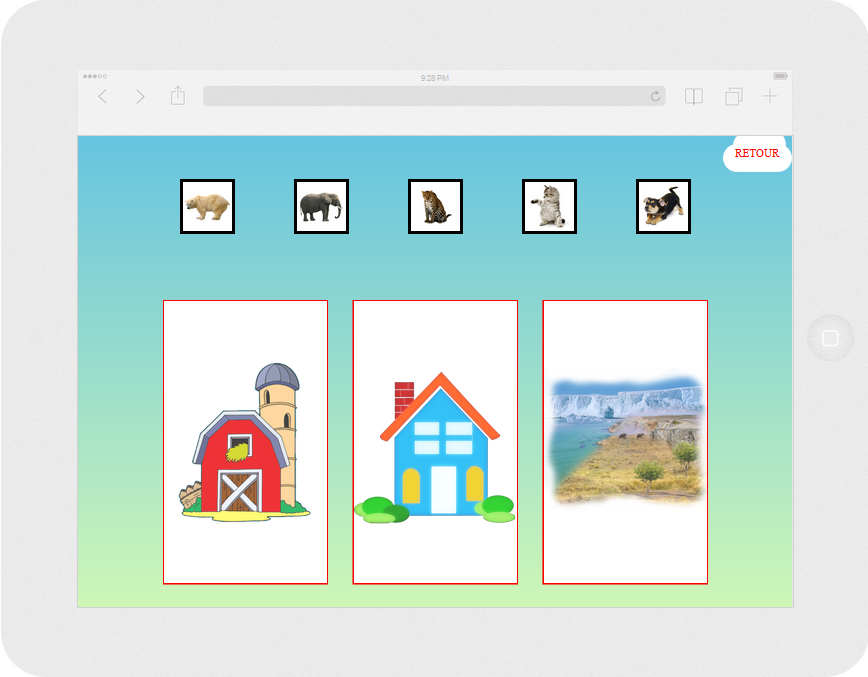
\includegraphics[width=1.0\textwidth]{zone7}
\vspace{0.5cm}\\


\section{Normes, standards et outils}

\subsection{Méthodes de conception}
\hspace*{0.6cm}Les méthodes de conception sont utilisées afin d'améliorer la qualité de la conception finale.
\vspace{0.5cm}\\
\hspace*{0.6cm}La norme \textbf{UTF-8} est utilisée afin de rendre les textes utilisés universels et fiables. En utilisant cette norme, le jeu devient utilisable et surtout réutilisable sur l'ensemble des ordinateurs à travers le monde.
\vspace{0.5cm}\\
\hspace*{0.6cm}Concernant l'élaboration du jeu, un style de conception ascendante a été choisi. Cette approche permet de s'appuyer sur des scripts réutilisables. Les niveaux étant sensiblement les même, on peux donc implémenter la base du jeu dans un script que nous réutiliserons dans l'ensemble des niveaux.

\subsection{Standards}

\hspace*{0.6cm}Les conventions de codage utilisées sont celles approuvées par le W3C. Les commentaires du Javascript qui sont dans le code suivent quant à eux les conventions de codage de Java.

\subsection{Langages de programmations}

\hspace*{0.6cm}L'\textbf{HTML5}, qui est la dernière révision majeure d'HTML, permet de représenter les pages web du jeu. Ce langage de balisage permet de structurer et de mettre en forme le contenu du jeu.\\
\hspace*{0.6cm}Le \textbf{CSS4} permet de décrire la présentation de notre jeu comme par exemple la taille de la police, la taille des images...\\
\hspace*{0.6cm}Le \textbf{JavaScript}, qui est le langage de programmation de script par excellence, permet d'ajouter de l'interaction au jeu. Ce langage permet entre autre d'interagir avec le clique lorsque l'on déplace les images des animaux.\\
\hspace*{0.6cm}Le \textbf{XML} permet dans le jeu d'ajouter ou de supprimer des animaux facilement sans modifier une seule ligne de code.

\subsection{Environnement et outils de développement}

\hspace*{0.6cm}Les différentes versions du jeu seront visionnables, téléchargeables sur un \textbf{GIT}, un logiciel de traitement de versions décentralisé. Cet outil permet aux membres de l'équipe de développer chacun une part du code final et de l'échanger facilement. Le code sera aussi visible par toute personne extérieur au projet. Un retour d'une personne extérieure serait un plus qui pourrait améliorer le jeu et/ou le code.
\vspace{0.5cm}\\
\hspace*{0.6cm}\textbf{JQuery}, une bibliothèque de Javascript, permet de faciliter la conception des scripts du jeu. Cette bibliothèque gr\^ace à des fonctions d'animations ou d'événement déjà implémenté permet donc de gagner du temps. Le développement est par conséquent accéléré.
\vspace{0.5cm}\\
\hspace*{0.6cm}Enfin, les images du jeu sont en grande partie issus d'Internet avec quelques modifications légères réalisé avec \textbf{Photoshop}. 

\subsection{Outils de test}
\hspace*{0.6cm}Pour tester le jeu, les différents navigateurs sur le marché (\textbf{Google Chrome, Mozilla Firefox, Safari, Opera, Internet Explorer}) seront amplement suffisants car ces derniers disposent d'outils permettant d'effectuer des tests et de déboguer les applications.\\
\hspace*{0.6cm}Pour les tablettes, \textbf{Opera Mobile Emulateur} est un outil puissant permettant de reproduire le comportement des tablettes et téléphones.\\

\section{Planning}

\begin{tabular*}{1.0\textwidth}{@{\extracolsep{\fill}} | c | l | }
  \hline
  & Choix du sujet\\
  & Création du dossier de conception\\
  Semaine 1 & Création du premier prototype\\
  & écriture de la documentation\\
  & Test de la version 1.0\hspace*{7.6cm}\\
  \hline
  & Ajout de nouvelles idées\\ 
  Semaine 2  & Amélioration du prototype jusqu'à la version finale\\
  & Test des versions intermediaires\\
  \hline
  Semaine 3  & Test et finalisation graphique\\
  \hline
  & Correctifs des détails\\
  Semaine 4-7 & Ajout de données\\
  & Tests finaux\\
  \hline
\end{tabular*}

\begin{center}
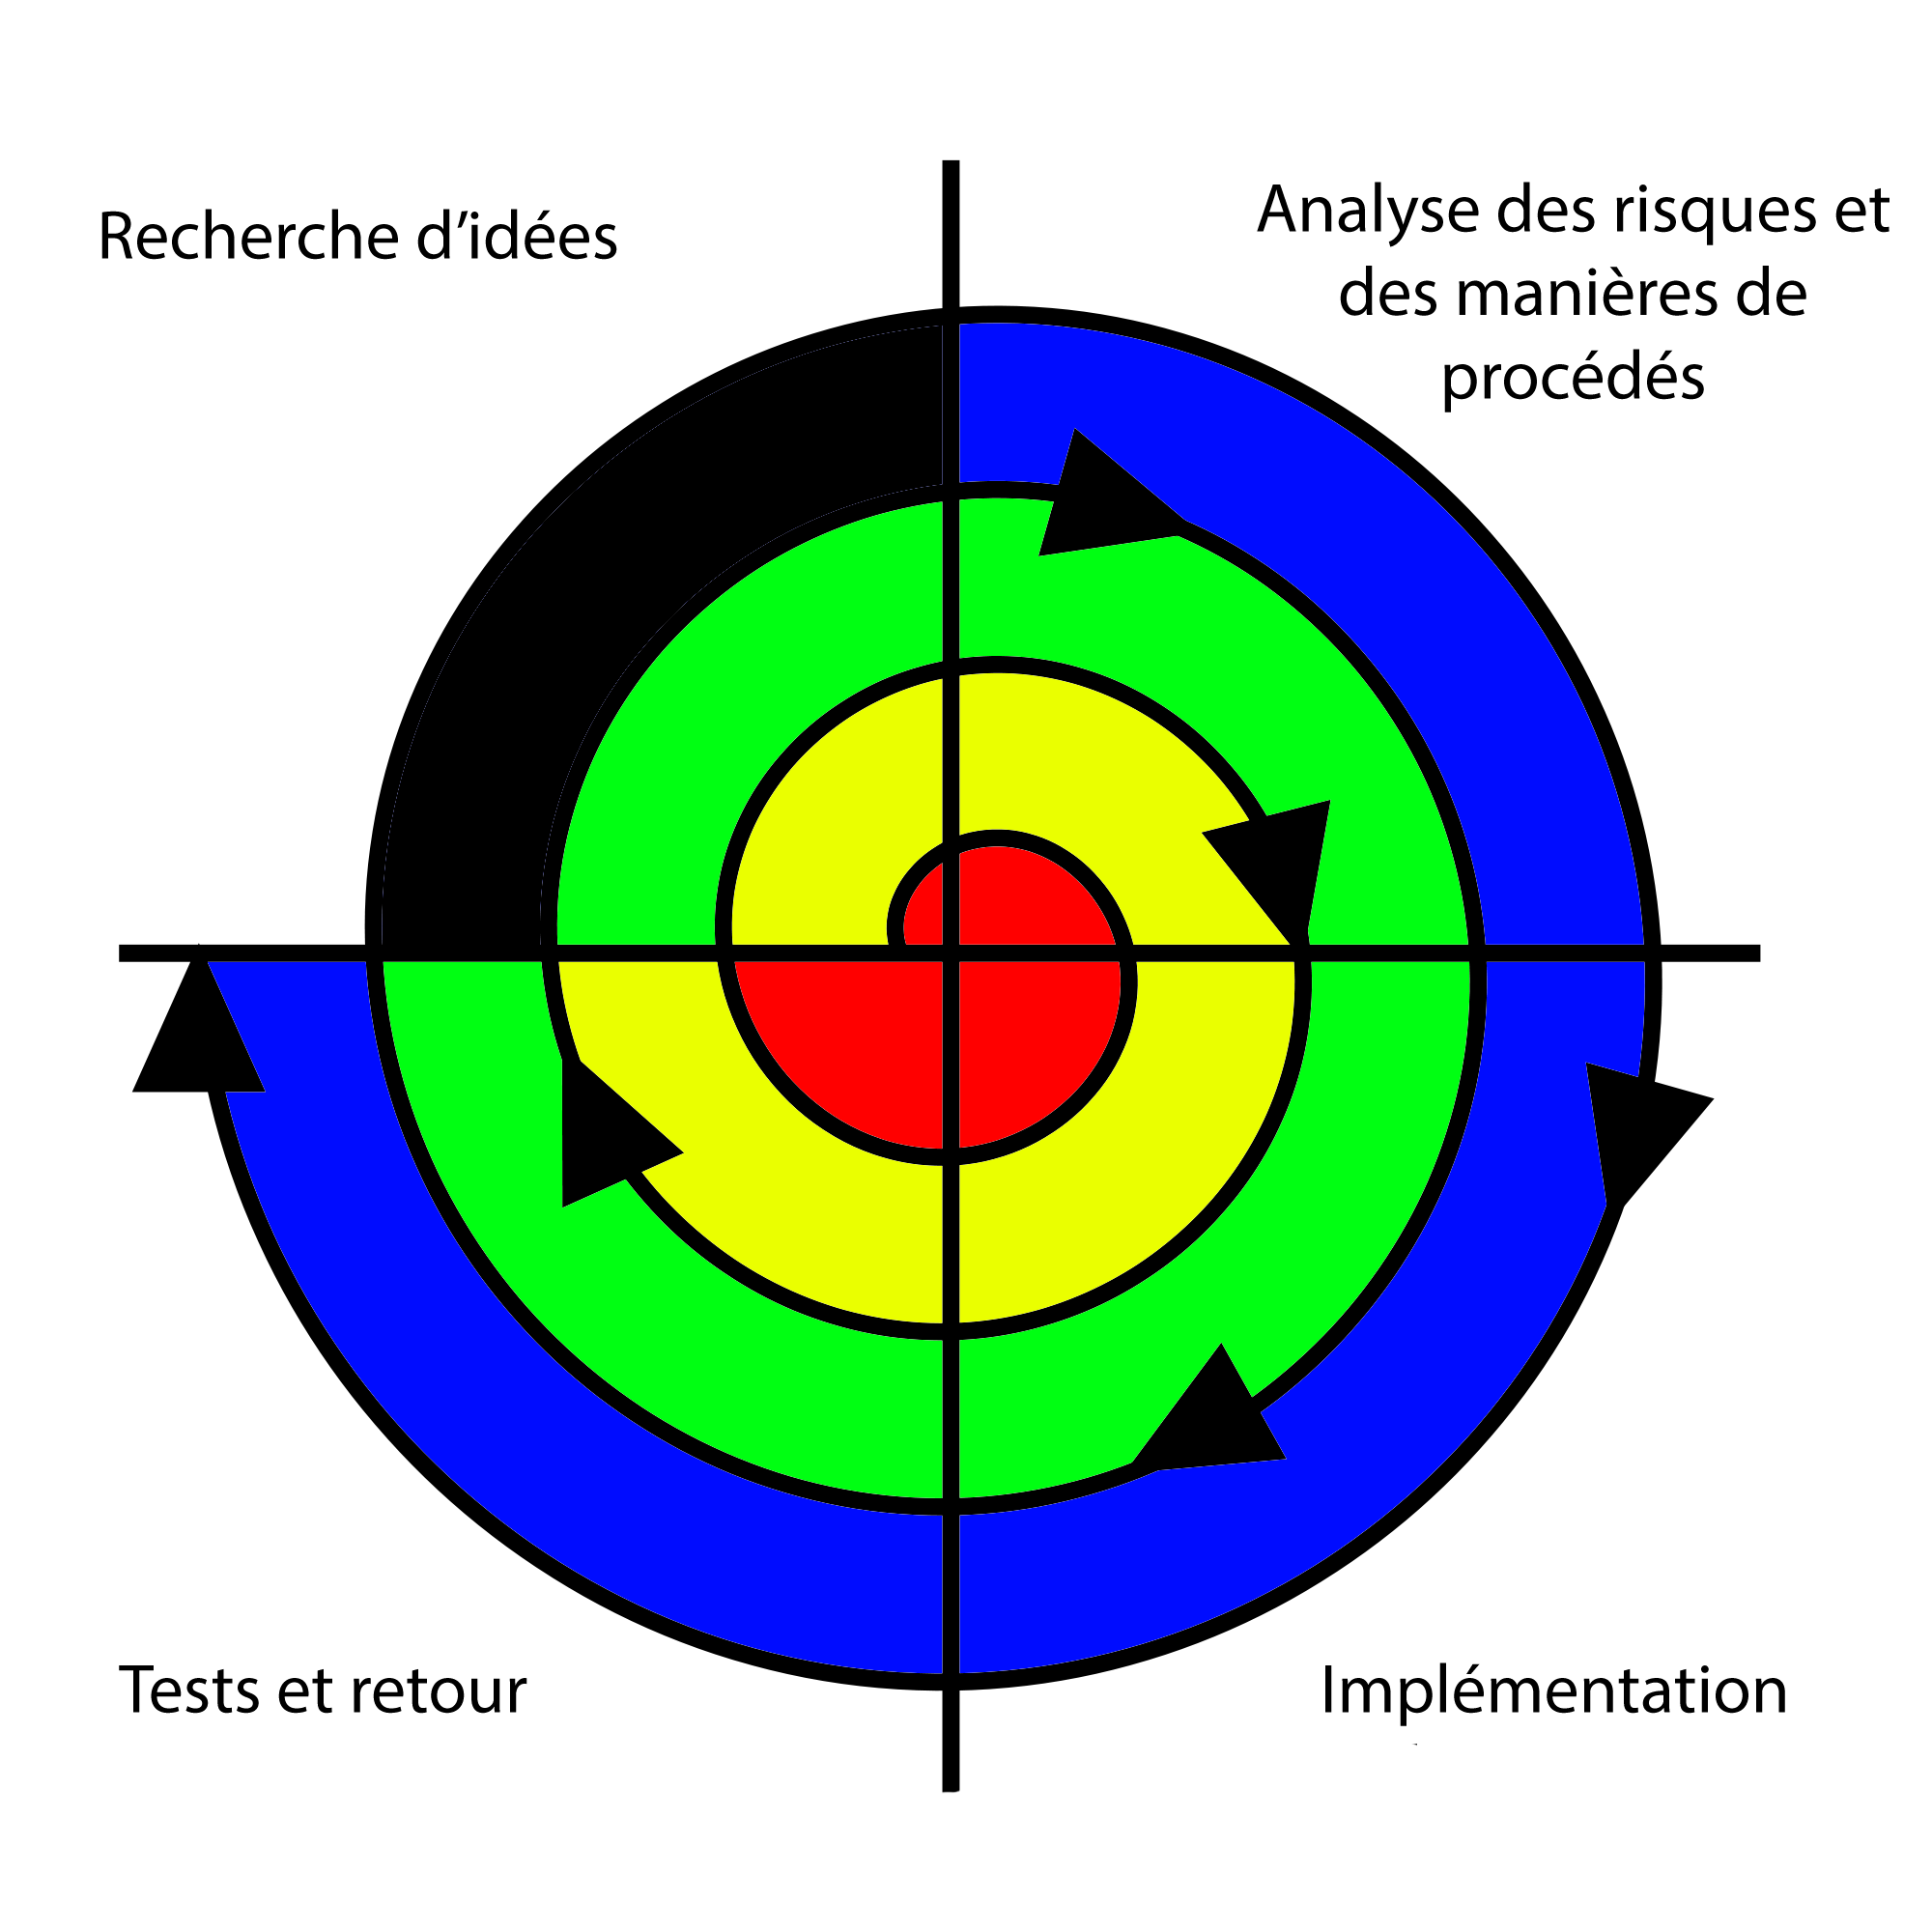
\includegraphics[width=0.6\textwidth]{spiral}\\
\end{center}

\textit{Le modèle spirale est un modèle de cycle de développement par implémentation de version successives, le cycle recommence en proposant un produit de plus en plus complet. On distingue quatres phases dans le déroulement du cycle en spiral :
\begin{itemize}
  \item Recherche d'idées
  \item Analyse des risques et des manières de procédés
  \item Implémentation
  \item Tests et retour
\end{itemize}
}
\vspace{0.7cm}
\hspace*{0.6cm}On suivra ainsi un modèle spirale pour le développement. En rouge, on retrouve notre première semaine de développement. à l'instant où ces lignes sont écrites, un premier prototype a été testé et produit. La semaine 2 en jaune sera donc de l'ajout d'idée avec l'implémentation et les tests qui iront avec. La semaine 3 en verte suivra le même schéma et pourra, suivant le déroulement du projet, se reproduire une ou deux fois. Puis la dernière semaine en bleu sera celle où plus aucun ajout ne sera toléré.\\


\end{document}